\documentclass{article}
\usepackage{tikz}
\usetikzlibrary{arrows.meta,positioning,calc,shapes.geometric}
\pagestyle{empty}
\begin{document}
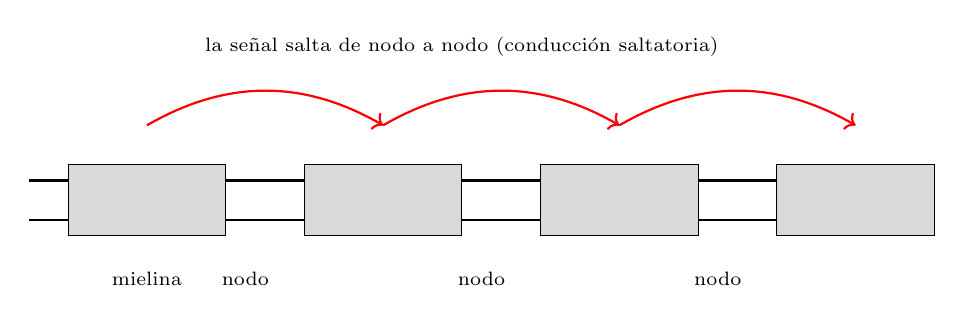
\begin{tikzpicture}

\draw[thick] (0,0) -- (11,0); \draw[thick] (0,-0.5) -- (11,-0.5);
\foreach \x in {0.5,3.5,6.5,9.5} {\draw[fill=gray!30] (\x,-0.7) rectangle (\x+2.0,0.2);}
\foreach \x in {2.5,5.5,8.5} {\node[font=\scriptsize] at (\x+0.25,-1.25) {nodo};}
\foreach \x in {1.5,4.5,7.5} {\draw[->, thick, red] (\x,0.7) to[bend left] (\x+3.0,0.7);}
\node[font=\scriptsize] at (5.5,1.7) {la señal salta de nodo a nodo (conducción saltatoria)};
\node[font=\scriptsize] at (1.5,-1.25) {mielina};

\end{tikzpicture}
\end{document}
